Galileo quería soltar una bola de madera y una bola de hierro desde una altura de 150 metros y medir el tiempo que tardan en caer.
Encontró una rampa con una inclinación de 15$^\circ$ por la que podía subir para llegar a una altura de 150 m.
En la figura \ref{fig:igor} se muestra una representación art\'istica que hizo su primo, Igor:
\begin{figure}[H]
    \begin{center}
        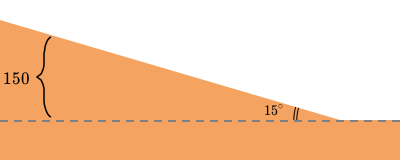
\includegraphics[width=0.5\textwidth]{../images/igor.png}
    \end{center}
    \caption{Vista transversal de la rampa donde Galileo hizo su experimento}
    \label{fig:igor}
\end{figure}
\textbf{¿Cuánto debe caminar Galileo a lo largo de la rampa?}\\
\textit{Redondea tu respuesta a la centésima más cercana.}